\chapter*{Introduzione}
\addcontentsline{toc}{chapter}{Introduzione}
Il mondo odierno è ormai pervaso dall'Intelligenza Artificiale. Uno dei settori di maggior interesse per la
ricerca in questo ambito è indubbiamente quello delle \emph{Self Driving Car}, ovvero
le macchine a guida autonoma. 
\begin{figure}
  \centering
  \parbox{5cm}{
  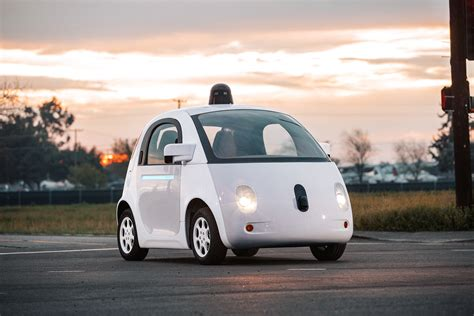
\includegraphics[width=5cm]{googlecar}
  \caption{Self driving car di Google.}
  \label{fig:google}}
  \qquad
  \begin{minipage}{5cm}
  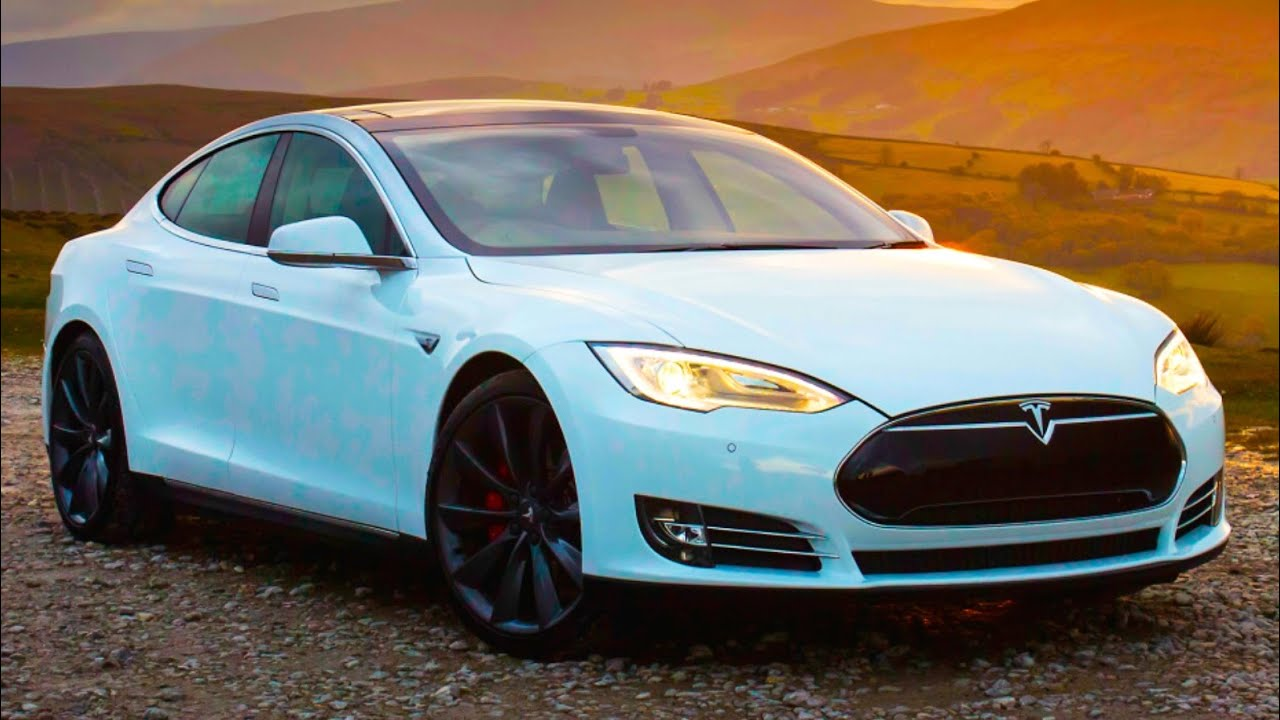
\includegraphics[width=5cm]{tesla}
  \caption{Self driving car di Tesla.}
  \label{fig:tesla}
  \end{minipage}
  \end{figure}
Grandi aziende quali \emph{Google} e \emph{Tesla} hanno già sviluppato
dei propri modelli  (Figura \ref{fig:google} e Figura\ref{fig:tesla}) e l'interesse in questo campo è sempre in  maggior crescita. Per poter funzionare correttamente, i veicoli a guida autonoma sfruttano il Machine Learning e le \emph{reti neurali}. Una macchina acquisisce immagini
dall'ambiente circostante attraverso varie camere e sensori. Queste immagini vengono passate a una rete neurale che, in base alle informazioni raccolte, decide l'azione da compiere (sterzare, accelerare, frenare ecc\dots).
L'utilizzo del Machine Learning ha permesso un notevole avanzamento nello sviluppo di questo settore ma  esistono ancora molte problematiche relative a sicurezza ed affidabilità.\\

Una vulnerabilità molto importante sono i cosiddetti \emph{Adversarial attacks}. Il meccanismo di questi attacchi è molto semplice:
Gli input della rete  subiscono una modifica volontaria, impercettibile a occhio umano ma in grado di causare errori di  classificazione.  Questi errori possono portare, ad esempio, una macchina ad accelerare quando
dovrebbe frenare. È fondamentale quindi studiare tali attacchi per verificare la robustezza dei modelli di apprendimento.
In questa Tesi abbiamo studiato, iniettato e verificato l'efficacia di  alcuni degli attacchi forniti dalla libreria python \emph{Adversarial Robustness Toolbox}. Gli attacchi scelti sono stati iniettato all'interno
di LearningByCheating, un modello di guida autonoma preaddestrato che gira sul simulatore di guida urbana Carla.
Il lavoro è così suddiviso:
\begin{itemize}
  \item \textbf{Capitolo 1:} Fondamenti teorici alla base dei sistemi intelligenti;
  \item \textbf{Capitolo 2:} Fondamenti di guida autonoma;
  \item \textbf{Capitolo 3:} Dependability e security;
  \item \textbf{Capitolo 4:} Strumenti utilizzati: vengono presentati \emph{l'Adversarial Robustness Toolbox} e il simulatore \emph{Carla};
  \item \textbf{Capitolo 5:} Il lavoro svolto: attacchi scelti e motivazioni, iniezione e risultati;
  \item \textbf{Capitolo 6:} Conclusioni e possibili sviluppi futuri.
  
\end{itemize}


